\documentclass[tikz]{standalone}
  \usepackage{tikz-network}
  \usetikzlibrary{patterns}


  % \usepackage{xcolor}
  % \pagecolor{lightgray!15}


  \def\firstcircle{ (0.0, 0.0) circle (1.5)}
  \def\secondcircle{(2.0, 0.0) circle (1.5)}
  \def\thirdcircle{ (1.0,-1.5) circle (1.5)}
  \def\rectangle{ (-1.5,-3.0) rectangle (3.5,1.0) }
  \colorlet{circle edge}{black}
  \colorlet{circle area}{blue!20}
  \tikzset{filled/.style={fill=circle area, draw=circle edge, thick},
      outline/.style={draw=circle edge, thick}}
  \setlength{\parskip}{5mm}


  \def\radius{1cm}
  \def\ratio{0.8}

  \def\circleA{(90:\ratio*\radius) circle [radius=\radius]}
  \def\circleB{(-150:\ratio*\radius) circle [radius=\radius]}
  \def\circleC{(-30:\ratio*\radius) circle [radius=\radius]}

  \tikzset{set label/.style={fill=white,circle,inner sep=.5mm}}

  \def\drawLabels{
  \node[set label] at (90:\radius+\ratio*\radius) {A};
  \node[set label] at (-150:\radius+\ratio*\radius) {B};
  \node[set label] at (-30:\radius+\ratio*\radius) {C};
  }
  \def\drawCaption#1{\node at (-90:2*\radius) {$#1$};}

  \def\drawVenn#1#2{
  \begin{tikzpicture}[baseline=0pt]
      \path[use as bounding box] (0,0) circle [radius=2.5*\radius];
      \draw \circleA \circleB \circleC;
      \begin{scope}[pattern=north west lines,pattern color=blue]
      #2
      \end{scope}
      \drawLabels
      \drawCaption{#1}
  \end{tikzpicture}%
  }

\begin{document}
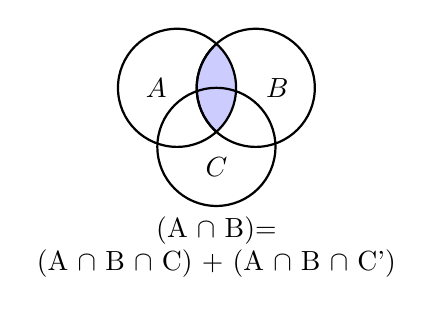
\begin{tikzpicture}[scale=0.5
]
\begin{scope}
        \clip \firstcircle;
        \fill[filled] \secondcircle;
    \end{scope}
    \draw[outline] \firstcircle  node[left]  {$A$};
    \draw[outline] \secondcircle node[right] {$B$};
    \draw[outline] \thirdcircle  node[below] {$C$};
    \node[anchor=north,align=center] at (current bounding box.south)
      {(A $\cap$ B)=\\(A $\cap$ B $\cap$ C) + (A $\cap$ B $\cap$ C')};
\end{tikzpicture}

\end{document}
